\subsection{M.PD.4 - Indice Gulpease}
\begin{figure}[H]
    \centering
    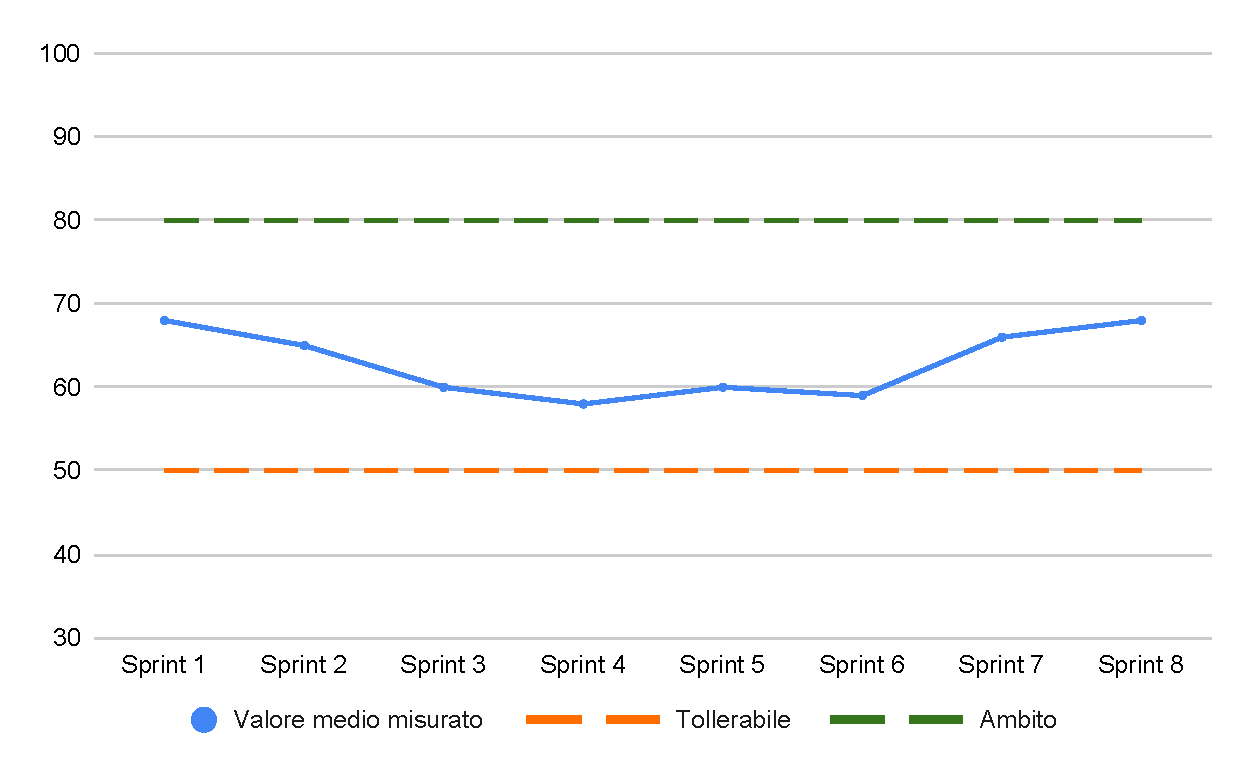
\includegraphics[width=\textwidth]{assets/indice_gulpease.pdf}
    \caption{M.PD.4 - Indice Gulpease}
\end{figure}

\par Il grafico riporta la media degli Indici Gulpease di tutti i documenti, sia interni che esterni. Il valore medio oscilla tra 55 e 75; ciò significa che i documenti sono comprensibili anche per chi possiede una licenza media. I valori più bassi sono stati rilevati nella fase centrale della \glossario{RTB}, poiché il team ha apportato modifiche sostanziali alla documentazione senza applicare un controllo rigoroso sulla leggibilità. Tuttavia, i valori misurati rientrano nella soglia di tollerabilità. Per quanto concerne i singoli documenti, l’\AdR\ ha evidenziato un indice di leggibilità inferiore rispetto agli altri, in quanto contiene frasi lunghe, specialmente nelle tabelle dei requisiti. Il \Gls\ ha un indice di leggibilità ancora inferiore ma entro i limiti tollerati; il basso punteggio è dovuto alla presenza di termini tecnici che richiedono una definizione approfondita. L’obiettivo del gruppo è di rielaborare, ove possibile, le porzioni più prolisse, riformulando il discorso e/o spezzando le frasi. Di seguito è riportato l’Indice Gulpease dei singoli documenti (per i verbali viene menzionato il valore medio).

\begin{table}[H]
    \centering
    \begin{tabular}{|c|c|}
        \hline
        \textbf{Documento} & \textbf{Indice Gulpease} \\
        \hline
        \PianoDiProgetto & 67\\
        \hline
        \PianoDiQualifica & 76\\
        \hline
        \NormeDiProgetto & 72\\
        \hline
        \AnalisiDeiRequisiti & 63\\
        \hline
        \Glossario & 50 \\
        \hline
        \emph{Verbali interni} & 77 \\
        \hline
        \emph{Verbali esterni} & 70 \\
        \hline
    \end{tabular}
    \caption{Tabella Indice Gulpease}
\end{table}